\section*{Del 1: Terminplanlegging}
	
	\begin{figure}[H]
		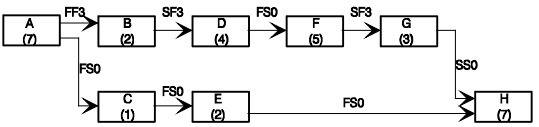
\includegraphics[width=\textwidth]{nettverk.png}
	\end{figure}

	\subsection*{Oppgave 1}
	{\bf Beregn alle tidligste og seneste tidspunkter samt total flyt for alle aktiviteter i 
	nettverket. Forutsett at ingen aktiviteter skal splittes. Før beregningene direkte på 
	nettverket.}

		\begin{table}[H]
			\begin{tabular}{ >{\centering\arraybackslash}p{2cm} | >{\centering\arraybackslash}p{2cm} | >{\centering\arraybackslash}p{1.5cm} | >{\centering\arraybackslash}p{1cm} | >{\centering\arraybackslash}p{1cm} | >{\centering\arraybackslash}p{1cm} | >{\centering\arraybackslash}p{1cm}}
				Aktivitet & Relasjon & Varighet & ES & LS & EF & LF \\ \hline
				A &  & 7 & 0 & 0 & 7 & 7 \\ \hline
				B & A: FF3 & 2 & 8 & 8 & 10 & 10 \\ \hline
				C & A: FS0 & 1 & 7 & 8 & 8 & 9 \\ \hline
				D & B: SF3 & 4 & 7 & 7 & 11 & 11 \\ \hline
				E & C: FS0 & 2 & 8 & 9 & 10 & 11 \\ \hline
				F & D: FS0 & 5 & 11 & 11 & 16 & 16 \\ \hline
				G & F: SF3 & 3 & 11 & 11 & 14 & 14 \\ \hline
				H & G: SS0, E: FS0 & 7 & 11 & 11 & 18 & 18 \\ \hline
			\end{tabular}
		\end{table}

		{\bf Total varighet:} 18 uker

		{\bf Kritisk sti:} A - B - D - F - G - H

		\begin{figure}[H]
			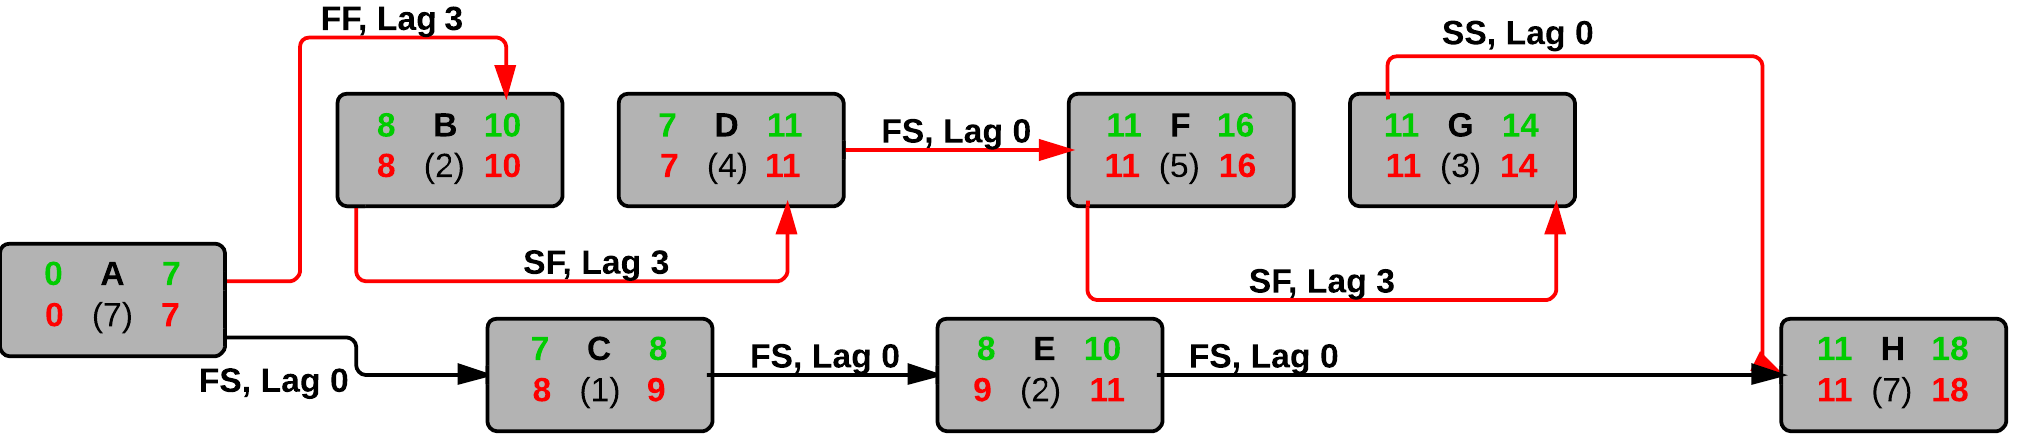
\includegraphics[width=\textwidth]{task1.png}
			\caption{Nettverk med beregna verdier + kritisk sti}
		\end{figure}

		
	\clearpage
	\subsection*{Oppgave 2}
		{\bf Hvilke konsekvenser for prosjektets ferdigtidspunkt får følgende tilfeller av endringer i akktivitetenes varigheter? Forklar kort hvordan du beregner konsekvensene i hvert tilfelle.}

		{\bf Tilfelle1: Aktivitet B forlenges 2 uker og aktivitet F forkortes 1 uke.}
		I dette tilfellet vil lengden av  prosjektet forkortes med 1 uke (fra 18 til 17 uker),
		samt at kritisk sti endres fra A-B-D-F-G-H til A-C-E-H. Måten vi beregnet dette på var
		å beregne alle verdier i stien som ble påvirket av endringene i B og F. Dette er stien
		A-B-D-F-G-H.
		
		\begin{figure}[H]
			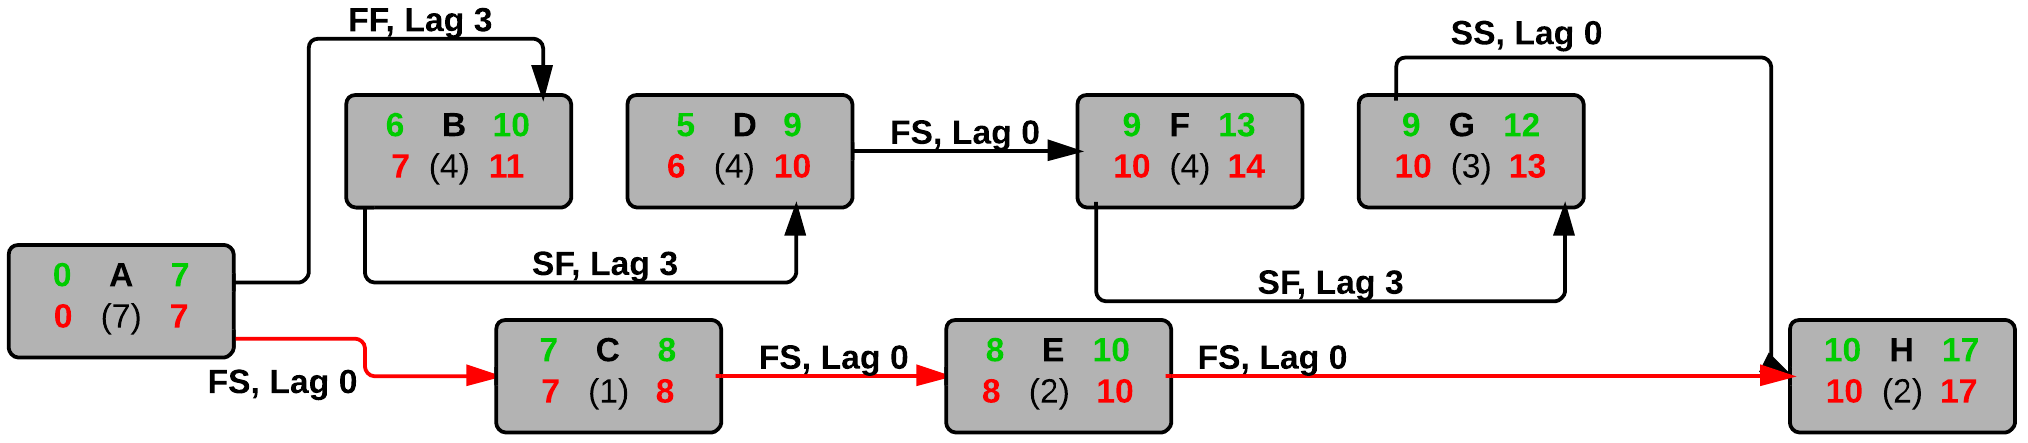
\includegraphics[width=\textwidth]{task2-1.png}
			\caption{Tilfelle 1}
		\end{figure}

		{\bf Tilfelle2: Alle aktiviteter forlenges 1 uke.}
		Ved en forlengelse av alle aktiviteter fikk prosjektet en lengre varighet på 4 uker 
		(fra 17 til 21 uker). Denne endringen medførte også en endring i kritisk sti fra 
		A-B-D-F-G-H til A-C-E-H. Måten vi beregnet dette på var at vi startet med forlengs beregning
		i nettverket og deretter regnet oss bakover. 

		\begin{figure}[H]
			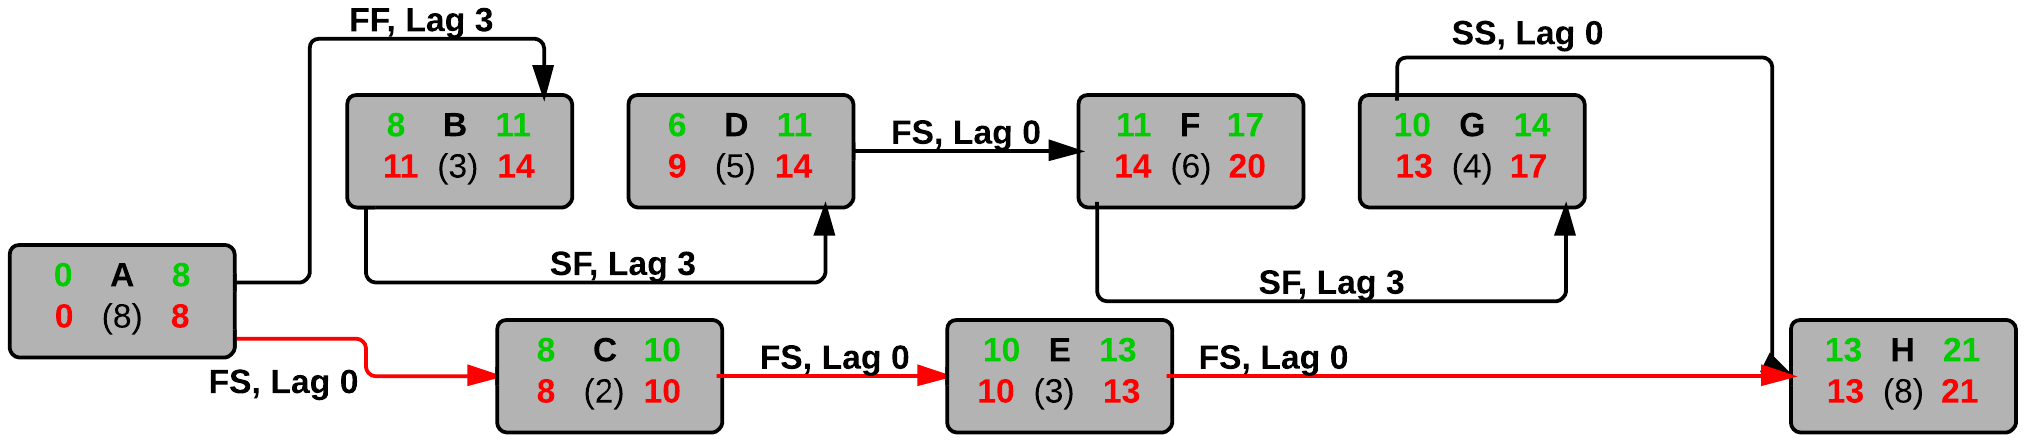
\includegraphics[width=\textwidth]{task2-2.png}
			\caption{Tilfelle 2}
		\end{figure}

	\clearpage
	\subsection*{Oppgave 3}

	\clearpage
	\subsection*{Oppgave 4}

		\begin{table}[H]
			\begin{tabular}{ >{\centering\arraybackslash}p{2cm} | >{\centering\arraybackslash}p{5cm} | >{\centering\arraybackslash}p{3cm}}
				Aktivitet & Beregning av TE & Varighet ($\approx$) \\ \hline
				A & (12 + 4 * 15 + 15)/6 = 16.17 & 16 \\ \hline
				B & (4 + 4 * 6 + 11)/6 = 6.5 & 7 \\ \hline
				C & (12 + 4 * 12 + 30)/6 = 15 & 15 \\ \hline
				D & (8 + 4 * 15 + 20)/6 = 14.67 & 15 \\ \hline
				E & (7 + 4 * 12 + 15)/6 = 11.67 & 12 \\ \hline
				F & (9 + 4 * 9 + 42)/6 = 14.5 & 15 \\ \hline
				G & (13 + 4 * 17 + 19)/6 = 16.67 & 17 \\ \hline
				H & (5 + 4 * 10 + 15)/6 = 10 & 10 \\ \hline
				I & (11 + 4 * 13 + 20)/6 = 13.83 & 14 \\ \hline
				J & (2 + 4 * 3 + 6)/6 = 3.33 & 3 \\ \hline
				K & (8 + 4 * 12 + 22)/6 = 13 & 13 \\ \hline
			\end{tabular}
		\end{table}

		{\bf Kritisk sti:} A-B-D-G-I-K

		{\bf Total varighet:} 82 uker

		\begin{figure}[H]
			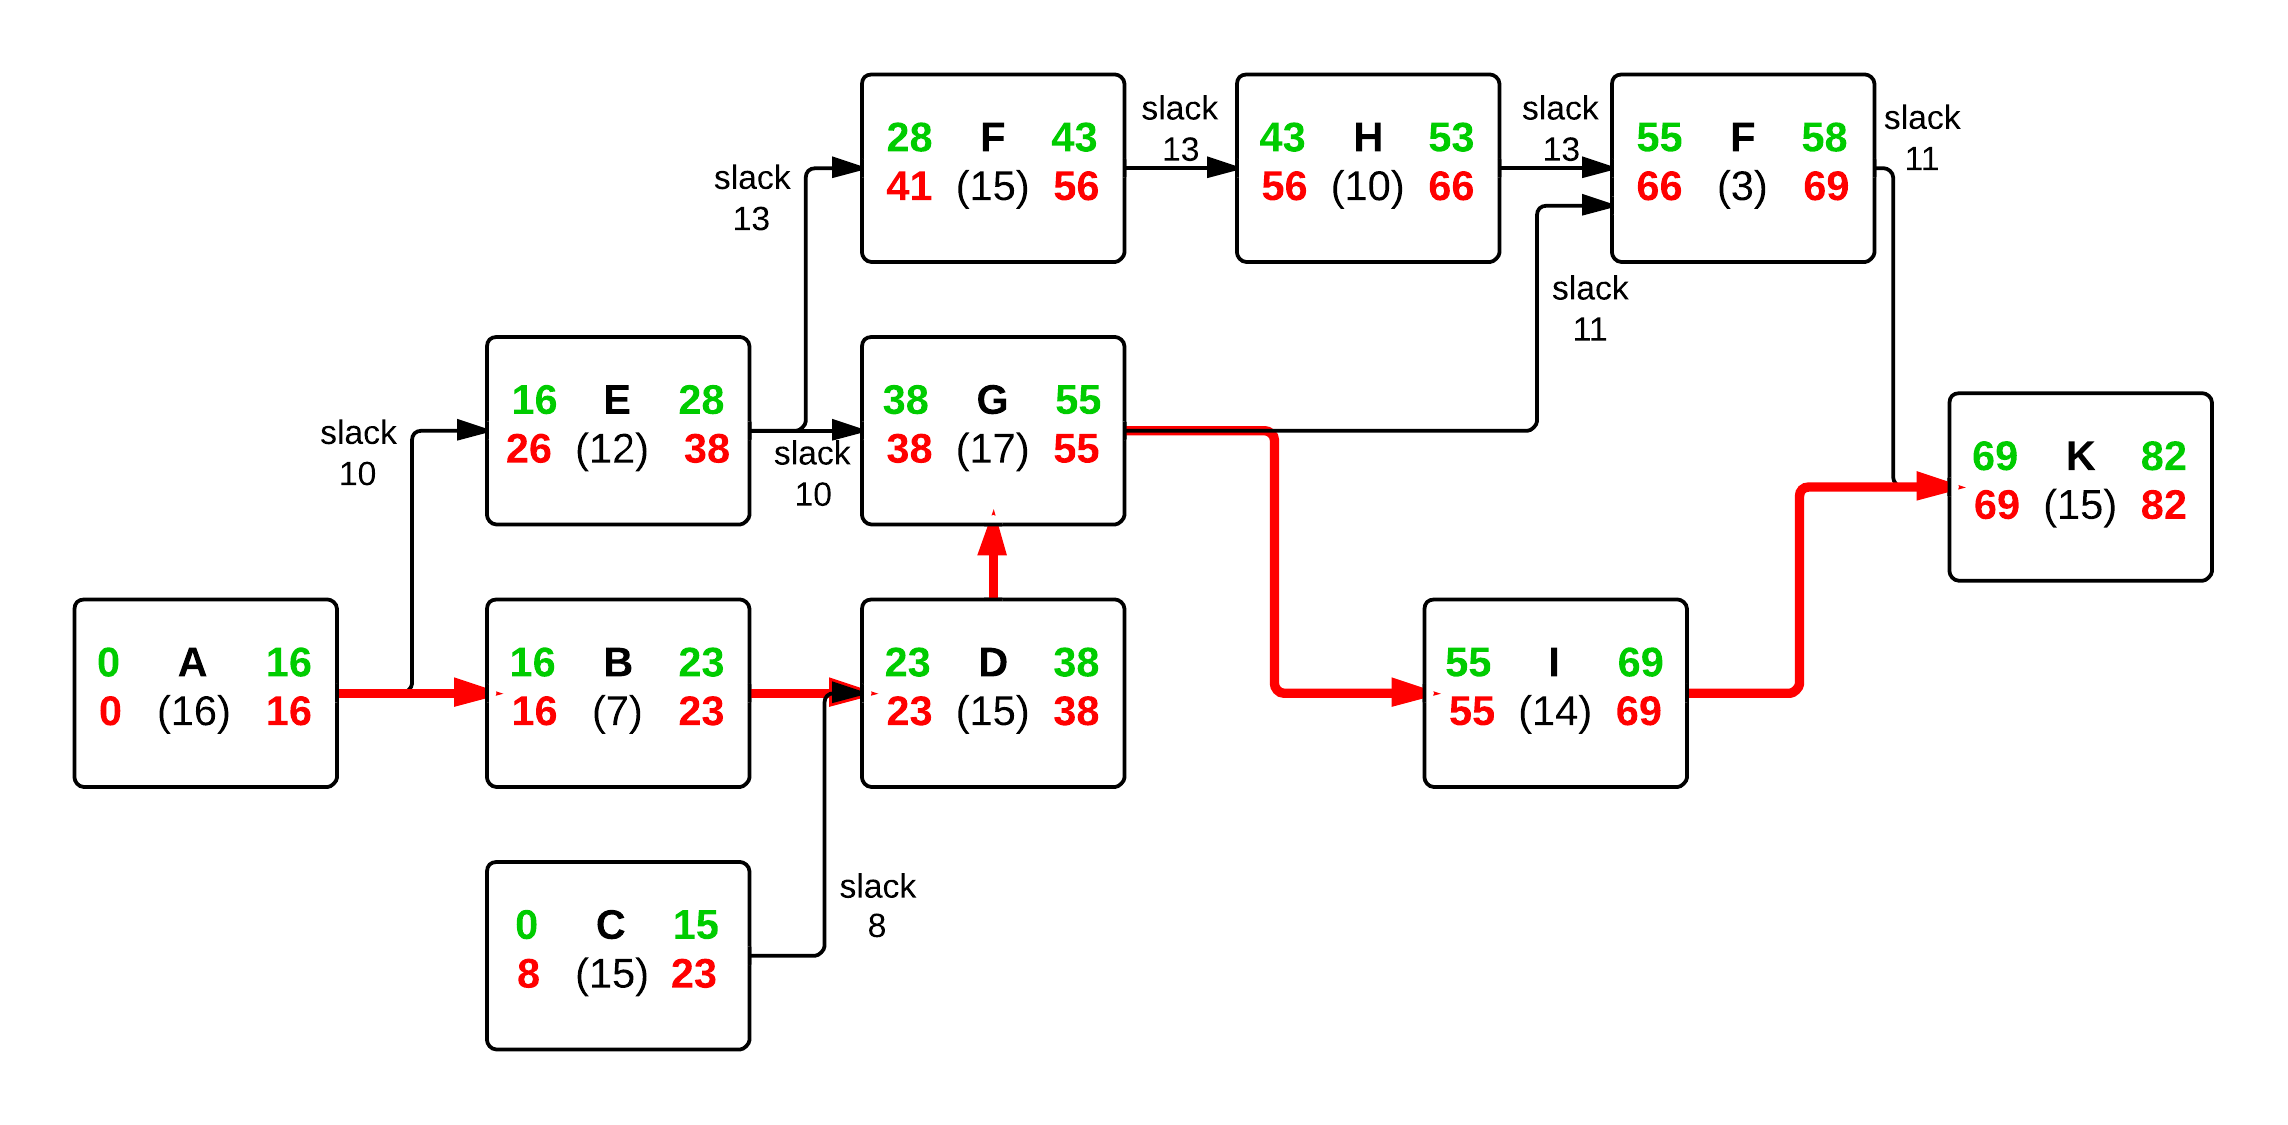
\includegraphics[width=\textwidth]{task4.png}
		\end{figure}

		{\bf a) Hvis vi antar at task E har tar 10 uker lengre tid enn planlagt. Hvilke konsekvenser får det?}

		Hvis vi ser på illustrasjonen av nettverket ser vi at selv om task E tar 10 timer ekstra
		så vil det ikke påvirke nettverket fordi den har en slack som er minst 10 uker ut til 
		aktiviteter som er avhengig av E. Det eneste som endres er at det ikke vil bli like mye slack og at 
		seneste start/slutt endres videre i nettverket som en konsekvens av endringen. Selve prosjektet
		vil ta like lang tid som før forsinkelsen, altså 82 uker. Kritisk sti forblir den samme. 

